\chapter{Evaluation}

The application is evaluated mainly based on user perspective.
The major aim for any performing user-based evaluation is to revolve around user-friendly and user-focused development\cite{Riihiaho_2018}. 

\textbf{Usability Testing: }\newline
Usability testing is performed with or without users by various techniques. In this project, we have done usability testing with users by carrying out various tasks in the application by selected users and analysing and observing the tasks carried out at several stages and collecting the results and resolving few bugs based on the test report\cite{Riihiaho_2018}.

Usability testing measures the overall quality and quantitative results of an application. It mainly focuses on the following parameters.
\begin{enumerate}
    \item Effectiveness
    \item Efficiency
    \item Accuracy
    \item User-Friendliness\cite{hamilton_2021}.
\end{enumerate}

\textbf{The Overall Process:}
 The overall process flows through several stages \cite{Calvin_Da_2012}
 \begin{enumerate}
 
 \item\textbf{ Participants Selection: }
 Testing was performed selecting 3 participants based on age, gender and location.
 Two participants in below 30 (with more experience of mobile) and one above 40 (with limited experience using mobile or system) with different genders and location were chosen to know the feedback.
  \item \textbf{Task Design: }
 Set of Tasks were designed to be carried out by all the users.
 The tasks include the overall functionalities and performance measures of the application.
 
 \begin{tabular}{ |p{2cm}|p{10cm}|p{10cm}|  }
\hline

\hline
Task\# &  Task Items \\
\hline

1 & Register new User \\
2 & User Login to application \\
3 & Go through UI Menus and Navigation to pages \\
4 & Newsfeed data access \\
5 & Like/Save/Favorite interactions \\
6 & View all interactions and understand personalization based on user details and interactions\\
7 & View User charts and data \\
8 & View Globe and news data and understand how to change category or country to access data\\
9 & Navigate to User profile \\
10 & Edit User profile \\
11 & Go to saved feeds and remove after reading if needed \\
12 & Land on any interested news  \\
13 & Validate the user details on registration  \\
14 & Understand recommendation process and view recommended items if any.\\
15 & Logout the application anytime.\\
16 & Is it easy to understand the application?\\
17 & Limited navigation and satisfied single page application purpose?\\
18 & How far the data is accurate in user profile and user charts?\\
19 & Is training required for users?\\
\hline
\end{tabular}

  \item \textbf{Task Analysis and Report: } 
  The tasks are carried out in order by all the participants and observed for tasks completion, duration to complete the tasks and provided help and support to complete in case required.
  Based on observation, below findings were made and reported accordingly. \newline
\textbf{ Collective findings of user-study:}\newline
\begin{tabular}{ |p{2cm}|p{12cm}|p{12cm}|  }
\hline

\hline
Task\# &  Limitations \\
\hline
1 & User registration not properly validated in front-end and unable to understand why the signup doesn't complete\\
2 & First name and last name not distinguished like in other applications. \\
3 & No option to search easily for any news item \\
4 & Unable to understand why like/save not working initially after landing on url. \\
5 & Some urls broken in menus\\
6 & Help Video or Tour for new users \\

\hline
\end{tabular}\newline
 \end{enumerate}
 
\textbf{Observations and bug fixes:}\newline
 Some of the issues observed in test reports are fixed and updated in the application and the respective screenshots are as below for reference.
 
 \begin{itemize}
     \item\textbf{ Missing Front-end validations:} 
     Though the validations are performed at the back-end, the user is unable to understand why the application is struck since there is no message at the front-end. So, the front-end validation is performed with sufficient messages for user to understand.
   \begin{figure}[h!]
    \begin{multicols}{2}
    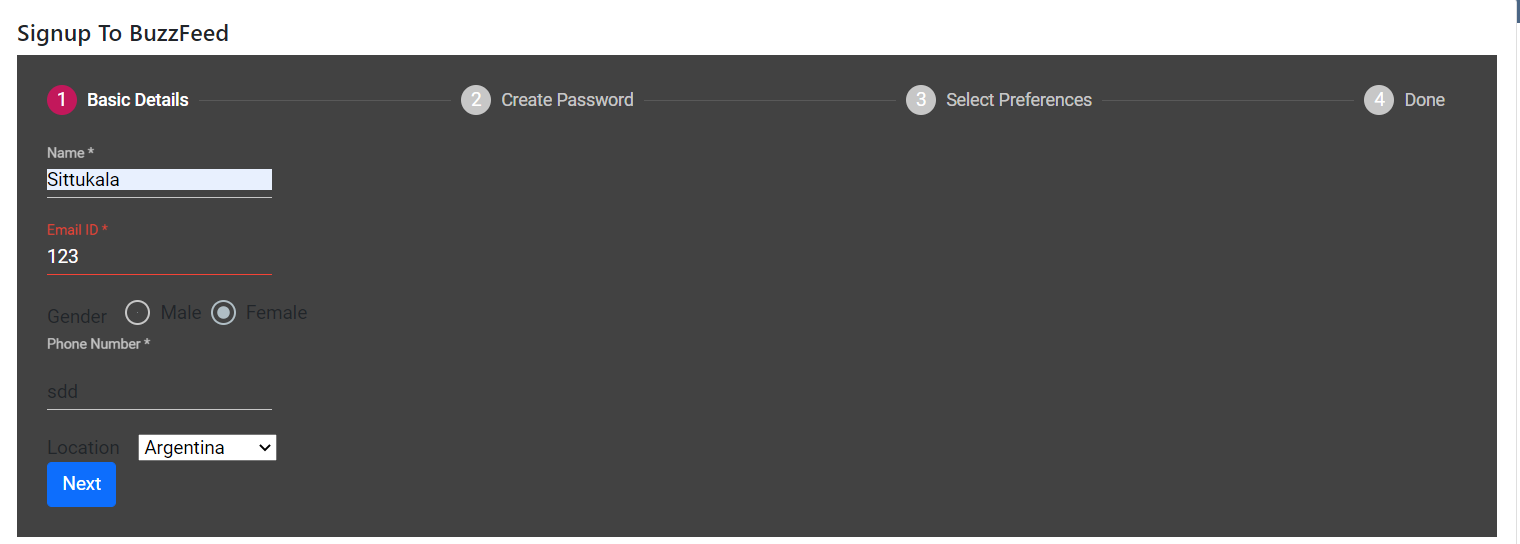
\includegraphics[width=\linewidth]{images/novalidation.PNG}\par 
    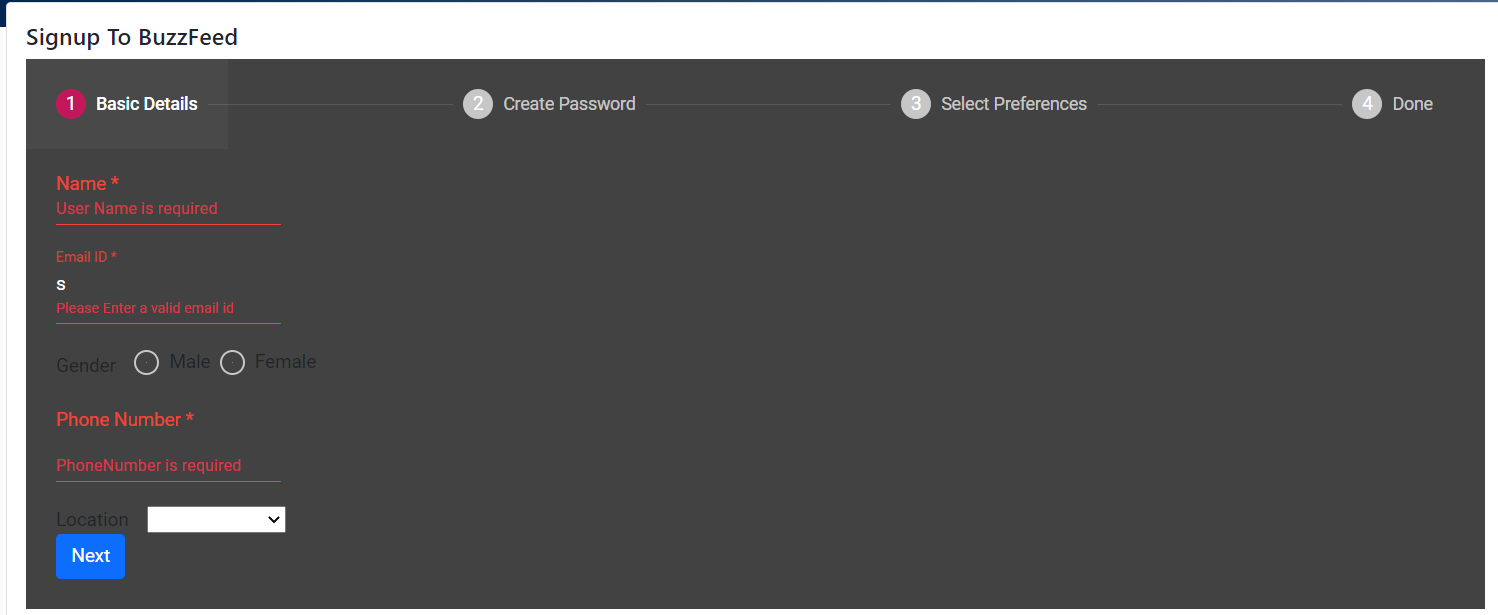
\includegraphics[width=\linewidth]{images/validation.PNG}\par 
    \end{multicols}
\centering \caption{Validation message}
\end{figure}

 \item\textbf{Interactions not working : } 
 The user reactions are not taken initially. The it was made clear it requires user login to allow interactions. But this should be properly conveyed to the users in a way they understand the pre-requisite to login. The popup appears if not logged in.
 
  \begin{figure}[h!]
    
    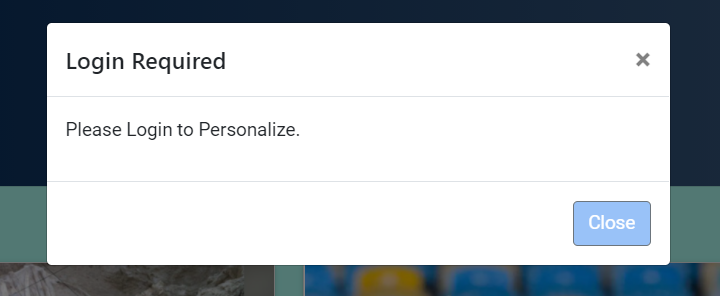
\includegraphics[width=\linewidth]{images/loginrequire.PNG}\par 
  
\centering \caption{Pre-requisite for interaction}
\end{figure}

\item\textbf{Search option : } 
Users were trying to search some news but there was no option to do, so it is added now.
 \begin{figure}[h!]
    \begin{multicols}{2}
    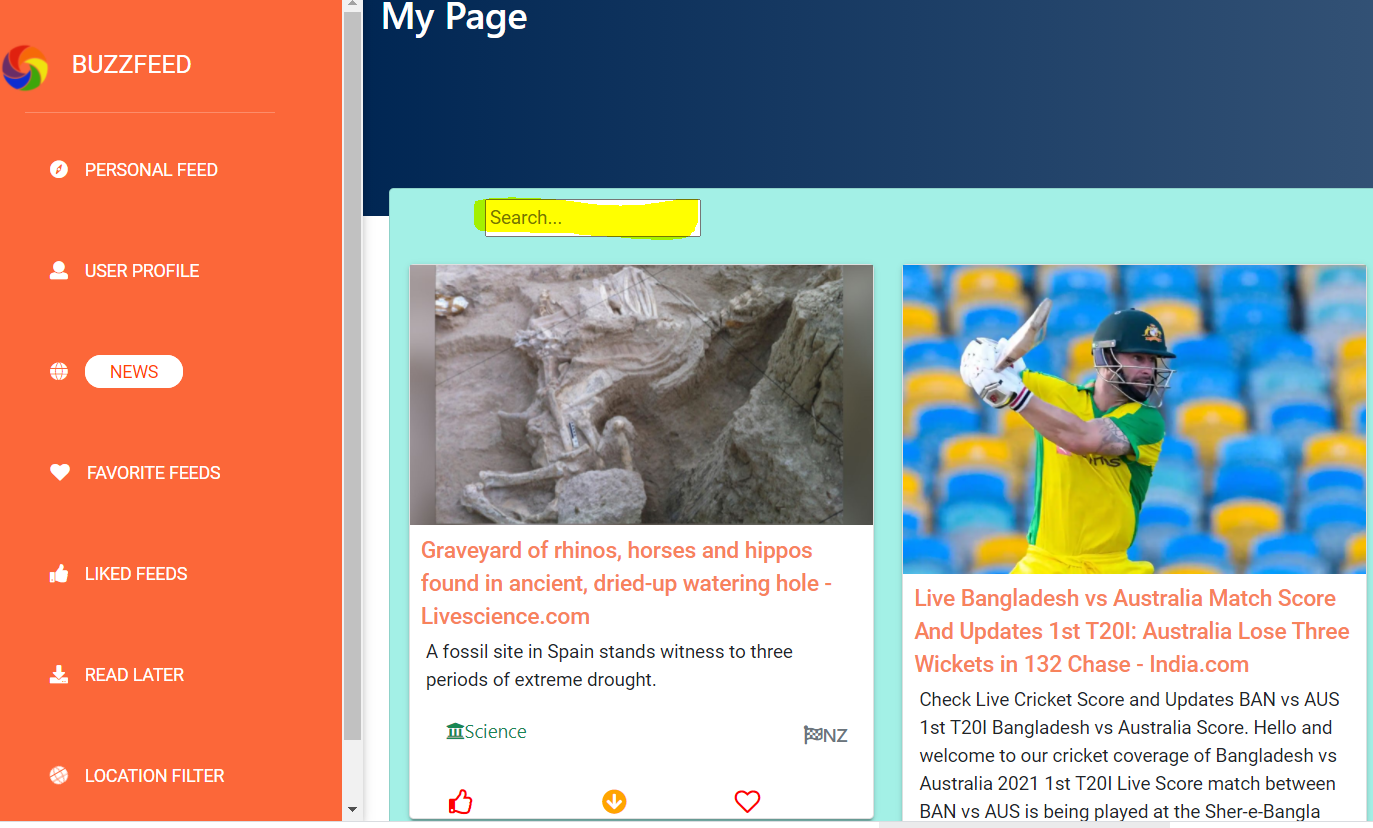
\includegraphics[scale = 0.5]{images/option.PNG}
    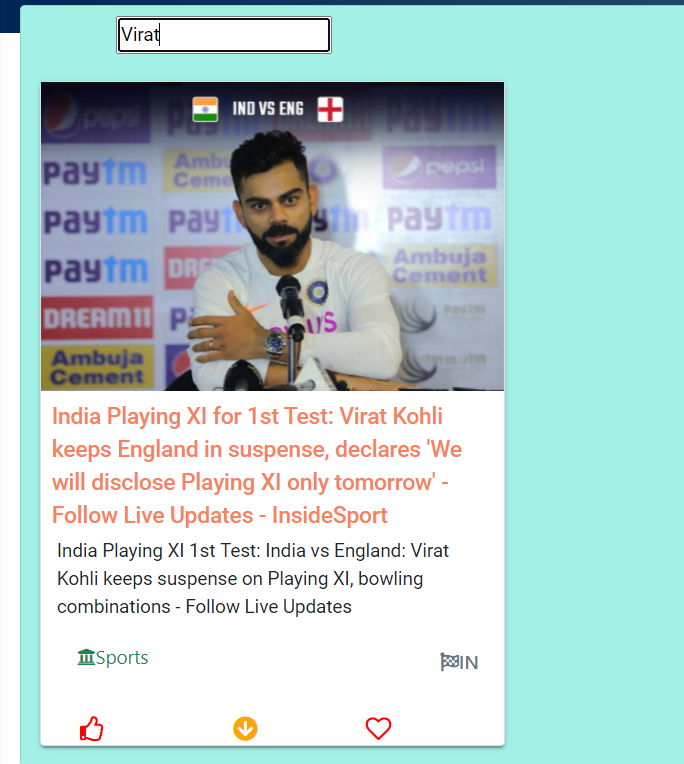
\includegraphics[scale = 0.5]{images/search.PNG} 
    \end{multicols}
\centering \caption{Search}
\end{figure}
 \end{itemize}
 

\textbf{Test-Driven Development:  }\newline
Apart from User testing, the application is also tested in-line with the development and made sure all the functionalities are tested for both positive and negative outcomes using Test Driven Development approach.
Developers intend to follow this approach incrementally writing unit test-cases and acceptance test-cases throughout the software development life-cycle \cite{NachiappanThirumalesh_2006}. 
The unit testing is mostly carried out using the Junit testing techniques for Java.

\textbf{Structure of TDD : } \newline
TDD runs incrementally with the rapid iterations of the below steps in sequence\cite{NachiappanThirumalesh_2006}.

 \begin{figure}[h!]
    \begin{center}
    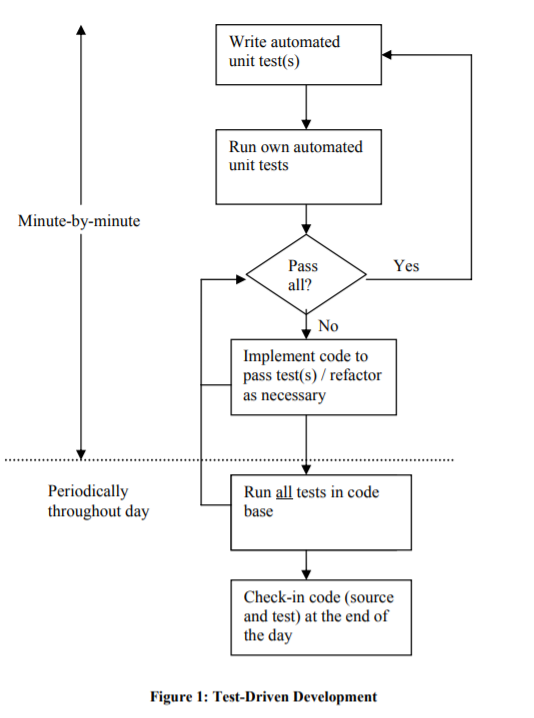
\includegraphics{images/TDD.PNG} 
  \end{center}
\centering \caption{Pre-requisite for interaction}
\end{figure}

\textbf{Successful test-suites : } \newline
 We have run several Junit test-cases for the functionalities and collected the test results. The test-cases are available for review under appendix with the sample test result screenshots here. 
 

 \begin{figure}[h!]
     \begin{center}
    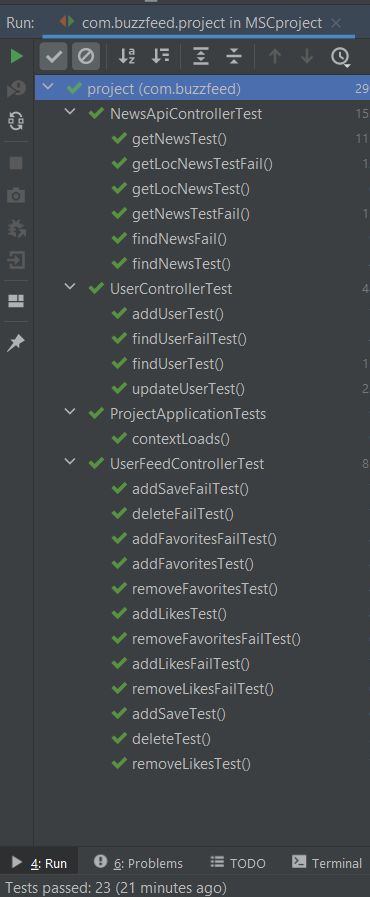
\includegraphics[scale=1]{images/testcases.PNG} 
  \end{center}
\centering \caption{Test suite}

\end{figure}

 
 



 
 